\documentclass[11pt]{article}
\usepackage{fullpage}
\usepackage{setspace}
\usepackage{amsmath}
\usepackage{fancyvrb}
\usepackage{enumerate}
\usepackage{listings}
\usepackage{pgfplots}
\usepackage{graphicx}
\usepackage{float}
\usepackage{multirow}
\usepackage[format=hang,labelsep=quad]{caption}
\usepackage{subfig}
\usepackage{array}
\usepackage{multirow}
\usepackage[final]{pdfpages}

\renewcommand\thesubfigure{\roman{subfigure}}


\begin{document}
\noindent\large{Math 5364}\\
\large{Data Mining 2}\\
\large{Homework 27}\\
\large{Mary Barker}

\begin{enumerate}
\item 
 The data set math5305Lab6Data.txt 
	contains 4 columns, Y, X1, X2, and 
	X3 respectively. Perform the 
	following using SAS.;

\begin{Verbatim}
	data math5305lab2;
	    infile '/folders/myshortcuts/sas_folder/math5305Lab6Data.txt' dlm=',';
	    input Y X1 X2 X3;
	proc print data=math5305lab2;
	run;
\end{Verbatim}

	\begin{enumerate}
		\item
		Fit the multiple regression model 
	
\begin{equation*}
Y_i = \beta_0 + \beta_1 X_{i1} + \beta_2 X_{i2} + \beta_3 X_{i3} + \epsilon_i;
\end{equation*}

\begin{Verbatim}
proc reg data=math5305lab2;
    model Y=X1 X2 X3;
    output out = mult_reg_model
    r = mult_reg_e
    predicted=mult_reg_pred;
run;

proc print data=math5305lab2;
run;
\end{Verbatim}

		\item 
		 What are the estimates 
			$\hat{\beta_1}, \hat{\beta_2},$ and $\hat{\beta_3}$?

			The estimated values for $\hat{\beta_i}$ for $i = 1, 2, 3$ are 
			17324, -22931, and 35741 respectively. 
		\item 
		Find the $t$-statistic and corresponding $p$-value for each of $X_1, X_2$ and $X_3$;

		The $t$-statistic and $p$-value for $X_1$ are: 13.48, and 0.0001.
		The $t$-statistic and $p$-value for $X_2$ are: -23.61, and 0.0001
		The $t$-statistic and $p$-value for $X_3$ are: 17.71, and 0.0001

		\item 
		Find the t-statistic and corresponding $p$-value for testing $\mathcal{H}_0: \beta_1 = \beta_2 = \beta_3 = 0$.

		\item 
		Find $R^2$ for this model

		The $R^2$ statistic for this model is 0.9066, and the adjusted $R^2$ is 0.9037.

		\item 
		Investigate normality of the residuals for this model using a qq-plot and the Shapiro-Wilk test.
	
\begin{Verbatim}
proc univariate data=mult_reg_model normal;
	var mult_reg_e;
	qqplot mult_reg_e;
run;
\end{Verbatim}
		The Shapiro-Wilk test gave a $p$-value of 0.0003. 

		\item
		Use the SPEC option to assess homoestadicity of the residuals;
		
\begin{Verbatim}
proc reg data=math5305lab2;
	model Y=X1 X2 X3/SPEC;
run;
\end{Verbatim}

		\item 
		Recall that $e$ is the vector of residuals and $\hat{Y}$ is the vector of predicted values. Produce the following 
		plots:
		\begin{itemize}
		\item $Y$ vs. $X_j$, $j$ = 1, 2, 3
		\item $Y$ vs. $\hat{Y}$
		\item $e$ vs. $X_j$, $j$ = 1, 2, 3
		\item $e$ vs $\hat{Y}$
		\end{itemize}

\begin{Verbatim}
proc plot data=mult_reg_model;
	plot Y * X1
		Y * X2
		Y * X3
		Y * mult_reg_pred
		mult_reg_e * X1
		mult_reg_e * X2
		mult_reg_e * X3
		mult_reg_e * mult_reg_pred;
run;
\end{Verbatim}

		\item Overall, do the typical linear regression 
			model assumptions appear to hold for this model?;

		The residuals do appear to be normally distributed, but the assumption of linearity does not hold. 
\end{enumerate}
\end{enumerate}
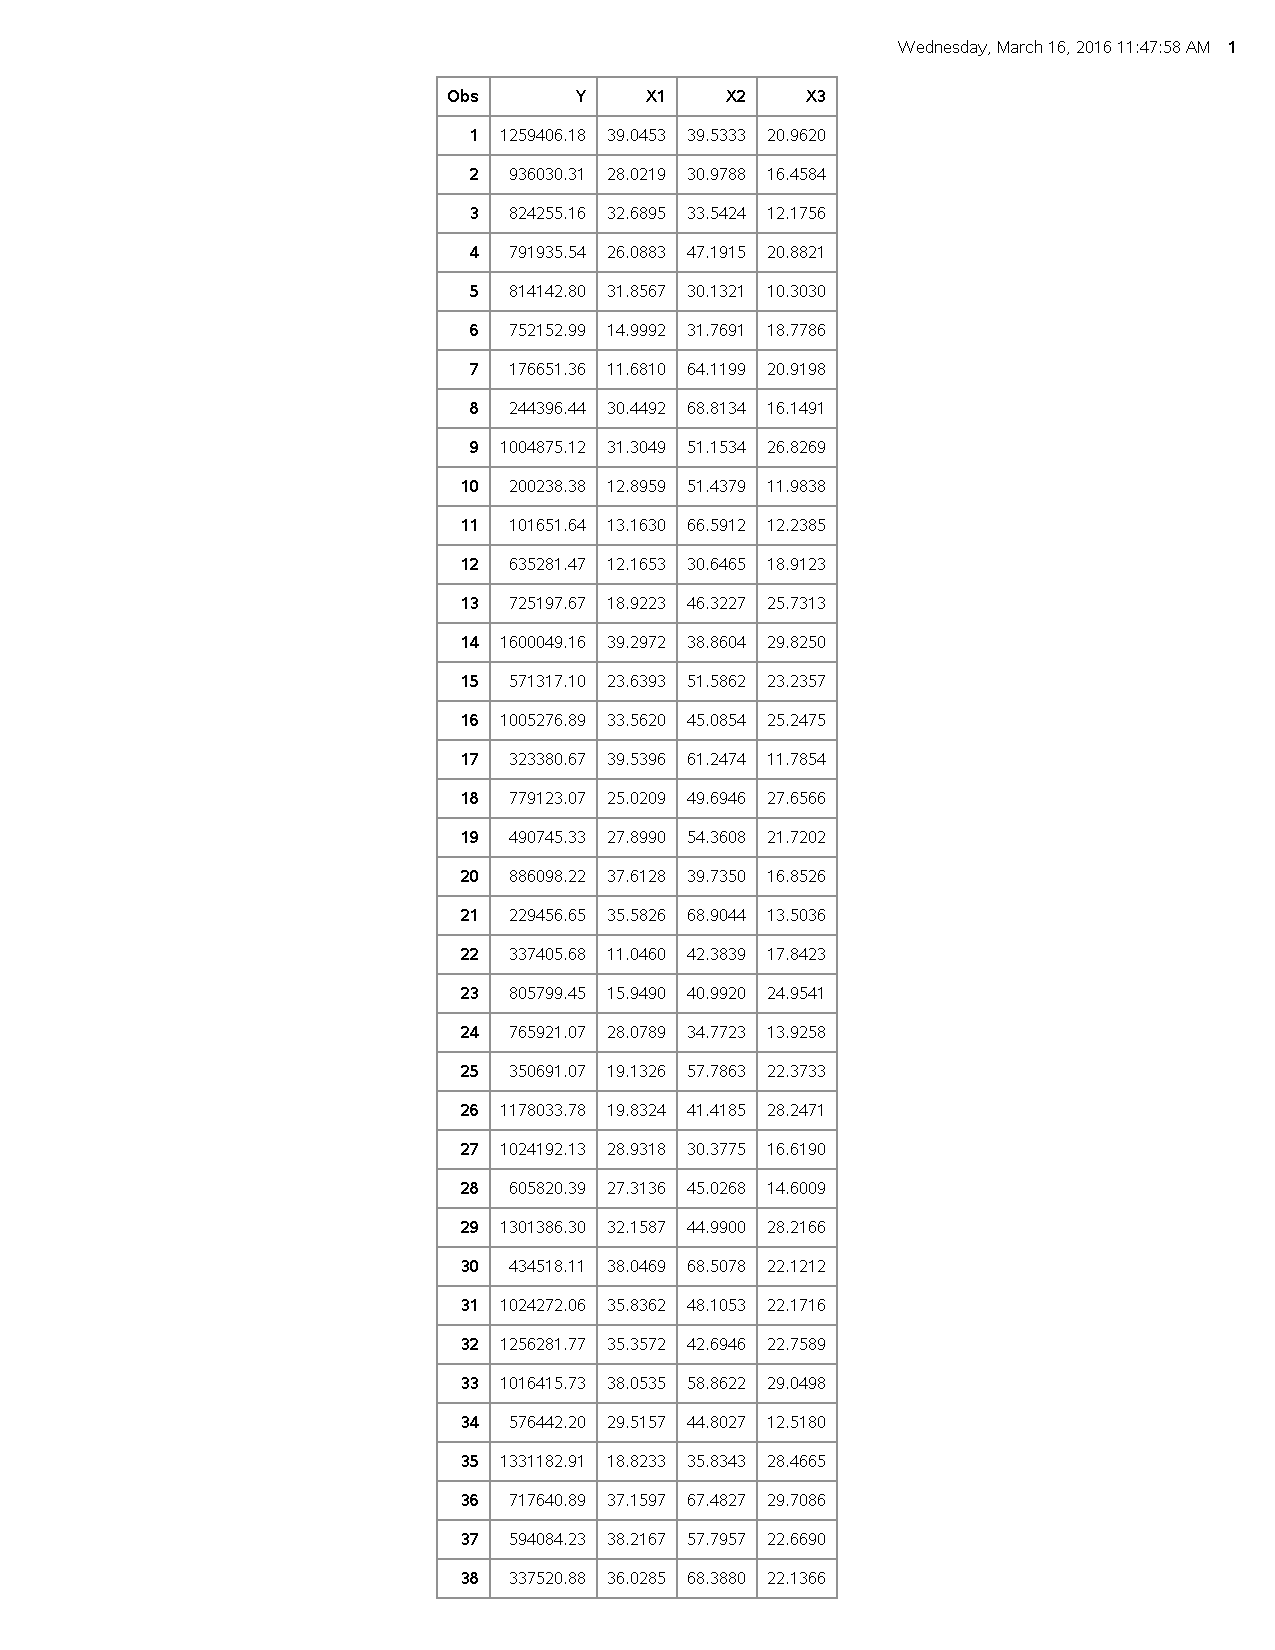
\includepdf[pages={1-}]{hw27_output.pdf}
\end{document}
